% Document class
% Document class
\documentclass[12pt,a4paper]{article}%

% Packages
\usepackage[utf8]{inputenc}%
\usepackage[T1]{fontenc}%
\usepackage{geometry}%
\usepackage{setspace}%
\usepackage{times}%
\usepackage{lipsum}% For dummy text
\usepackage{graphicx}%
\usepackage{fancyhdr}%
\usepackage{titlesec}%
\usepackage{tocloft}%
\usepackage{amsmath,amssymb}%
\usepackage{caption}%
\usepackage{subcaption}%
\usepackage{booktabs}%
\usepackage{hyperref}%
\usepackage{natbib}%

% Geometry
\geometry{
  a4paper,
  left=3cm,
  right=2cm,
  top=2cm,
  bottom=2cm
}%

% Line spacing
\onehalfspacing%

% Page numbering
\pagestyle{fancy}%
\fancyhf{}%
\rfoot{\thepage}%

% Section formatting
\titleformat{\section}[block]{\normalfont\Large\bfseries}{\thesection}{1em}{}%
\titleformat{\subsection}[block]{\normalfont\large\bfseries}{\thesubsection}{1em}{}%

% Table of contents formatting
\renewcommand{\cftsecleader}{\cftdotfill{\cftdotsep}}%


\begin{document}

\begin{titlepage}
  \centering
  \vspace*{5cm}
  {\Huge \textbf{[Your Thesis Title]}}\\[2cm]
  {\large Master Thesis presented to the Department of Economics at the}\\
  {\large Rheinische Friedrich-Wilhelms-Universität Bonn}\\[1cm]
  {\large In Partial Fulfillment of the Requirements for the Degree of Master of Science (M.Sc.)}\\[2cm]
  Supervisor: [Supervisor Name] \\[0.5cm]
  Submitted in [Month Year] by: \\[0.2cm]
  [Your Full Name] \\[0.2cm]
  Matriculation Number: [Your Matriculation Number]
  \vfill
\end{titlepage}

% Table of Contents
\tableofcontents
\thispagestyle{empty}
\newpage

% Start of main text
\pagenumbering{arabic}
\setcounter{page}{1}


\section{Introduction}
\lipsum[1-2]

\section{Literature Review}
Climate change mitigation policies are heavily influenced by the development trajectories of nations and their respective stages of economic growth, as outlined in the fifth assessment report by the Intergovernmental Panel on Climate Change (IPCC, 2007). According to emission estimates for 2023 provided by the EDGAR database, global greenhouse gas (GHG) emissions increased by 1.9\% compared to 2022, reaching 53.0 Gt CO2eq. The major contributors to global GHG emissions in 2023 were China, the United States, India, the European Union (EU27), Russia, and Brazil, which together accounted for 62.7\% of the total global emissions. Carbon dioxide (CO2) produced by human activities remains the largest driver of global warming, with its concentration in the atmosphere having risen by 48\% above pre-industrial levels (before 1750) by 2020. The primary sources of CO2 emissions include the combustion of coal, oil, and natural gas, deforestation, livestock farming, the release of fluorinated gases from industrial equipment, and the use of nitrogen-based fertilizers (Weber \& Matthews, 2008). These activities have led to more frequent and severe weather events, including heatwaves and droughts, that are impacting regions around the world. In 2024, the United States experienced 27 weather and climate-related disaster events, each resulting in losses exceeding \$1 billion (NOAA, n.d.).
\vspace{5pt}
The growing acknowledgment of global warming as a significant threat has prompted international initiatives aimed at reducing greenhouse gas (GHG) emissions. These initiatives rely on accurate assessment and reporting of GHG emissions to inform climate policies (IPCC, 2007). Households account for 17\% of total global carbon dioxide (CO2) emissions, underscoring their critical role in addressing climate change. Understanding and mitigating residential contributions to greenhouse gas (GHG) emissions require prioritizing the household carbon footprint, a vital measure of emissions stemming from residential consumption (Du \& Zhong, 2024). Several methodologies are available for estimating GHG emissions, with the concept of carbon footprint gaining significant attention (Guinee, 2011). A carbon footprint is defined as the total GHG emissions caused directly and indirectly by an individual, organization, event, or product, traditionally calculated by summing emissions from every stage of a product or service's life cycle (Center for Sustainable Systems, 2024). Among the available methodologies, the GHG Protocol has emerged as a widely used framework for corporate GHG reporting, considering direct and indirect emissions resulting from household consumption. However, this method has limitations, such as double-counting and restricted adjustments for market dynamics (WBCSD, 2004). 
\vspace{5pt}

Another widely used approach is the Input-Output Analysis (IOA) method, a top-down model that calculates carbon footprints by analyzing monetary transactions between activities and extending them to an environmental level through greenhouse gas (GHG) emissions. This approach, known as Environmentally Extended Input-Output Analysis (EEIO), provides a macro-level view of the environmental impacts of economic activities (Encyclopedia of Ecology, 2019). For instance, a study using EEIO to examine the carbon footprints of Australian equity investments and Socially Responsible Investments (SRI) demonstrated that applying SRI criteria significantly reduces the carbon footprint of equity portfolios. This highlights equity investments as a major driver of economic activity and a crucial lever in advancing a sustainable economy (Chard, 2024).
\vspace{5pt}

Another frequently used method for calculating carbon emissions is the Emission Factor (EF) method. According to the Intergovernmental Panel on Climate Change (IPCC, 2019), the formula for estimating GHG emissions is:
\[
\text{GHG Emissions} = \text{Activity Data (AD)} \times \text{Emission Factor (EF)}
\]
Here, Activity Data (AD) refers to the scale of production or consumption activities that result in GHG emissions, such as fossil fuel use or electricity consumption. The Emission Factor (EF) represents the amount of GHG emitted per unit of activity, such as the emissions per liter of fuel burned or per kilowatt-hour of electricity consumed. Life Cycle Assessment (LCA) is a highly sophisticated tool for examining the environmental impact of products and services. It offers a holistic evaluation, tracing environmental consequences across every stage of a product's existence, from the extraction of raw materials to its final disposal—often described as a "cradle-to-grave" approach. By analyzing phases such as production, distribution, usage, and end-of-life processes, LCA quantifies resource use, greenhouse gas emissions, and pollution affecting air, water, and soil systems (Global Climate Initiatives, 2023). A study leveraging LCA and household survey data provided precise calculations of carbon footprints by capturing emissions associated with daily consumption, household production activities, and the supply chain of consumed goods (Peng, 2021).

\vspace{5pt}

The model by Hakenes and Schliephake (2024) offers a fresh perspective on carbon footprint estimation by addressing the shortcomings of traditional static models. This consequentialist approach integrates market behaviors and industry-specific responses to provide a more dynamic and realistic analysis of household emissions. It highlights the connection between individual consumer decisions and broader emission outcomes, accounting for variables such as price elasticity and interdependencies between industries in both product and financial markets. By separating direct emissions tied to household activities from spillover effects influencing other sectors, this model delivers a more detailed and actionable understanding of household contributions to carbon emissions, paving the way for tailored climate strategies.


\section{Methodology}
\lipsum[3-4]

\section{The GHG Protocol}
The Greenhouse Gas (GHG) Protocol is a globally recognized standard for accounting and reporting greenhouse gas emissions. Developed in the late 1990s through a collaboration between the World Resources Institute (WRI) and the World Business Council for Sustainable Development (WBCSD), the GHG Protocol was officially launched in 2001 with the primary aim of providing a consistent and comprehensive framework for emissions accounting across corporate and public sectors. Over the years, its importance has grown significantly, with subsequent expansions such as the development of the GHG Protocol Scope 3 Standard in 2011, which broadened the accounting boundary to include indirect emissions across a company’s or household’s value chain. The historical motivation behind its creation was rooted in the need for greater transparency and comparability in emissions disclosures, especially as climate policy instruments and stakeholder expectations became increasingly sophisticated.

The GHG Protocol is structured around three main scopes of emissions, each delineating a distinct layer of responsibility and source attribution. Scope 1 covers direct emissions from sources that are owned or controlled by the reporting entity, such as the combustion of fuels in household-owned vehicles or heating systems. Scope 2 includes indirect emissions associated with the generation of purchased electricity, steam, heating, or cooling consumed by the household but produced off-site. Scope 3 is the broadest category, encompassing all other indirect emissions that occur as a consequence of the household’s activities but are not directly controlled by it. These include emissions from the production and transport of goods and services consumed by the household, as well as those associated with financial investments and capital goods.

The principal reason for employing the GHG Protocol in household-level emissions analysis lies in its capacity to provide a standardized and granular approach to calculating emissions across different dimensions of behavior. It allows for a full inventory of climate impacts arising from everyday life—from fueling a car to investing in equity portfolios. Additionally, the protocol facilitates benchmarking across time and geography, making it possible to compare the carbon intensities of different households or regions. This is particularly valuable for policy-making, where a reliable basis for comparison is needed to design effective incentives, taxes, or subsidy programs aimed at reducing emissions.

Households may apply the GHG Protocol methodology when they aim to understand the full extent of their carbon footprint, either for personal environmental awareness or to comply with voluntary disclosure programs. It is also useful in academic and policy research, where household-level emissions data feed into broader simulations of national carbon inventories or help evaluate the effectiveness of climate policies. Moreover, with the rise of ESG (Environmental, Social, and Governance) investing, households are increasingly motivated to assess not only their consumption patterns but also the environmental implications of their financial choices. The GHG Protocol's inclusion of Scope 3 investment-related emissions is thus particularly timely and relevant.

The benefits of using the GHG Protocol are manifold. First, it ensures methodological consistency by offering a clearly defined structure and a set of standard emission factors that can be applied universally or tailored regionally. This consistency is crucial for the comparability of results and for building credible datasets over time. Second, the protocol is transparent and traceable. It encourages users to document the sources of their activity data and the emission factors applied, thus allowing for auditing, replication, and critical scrutiny. Third, its structure is flexible enough to accommodate varying levels of data availability and resolution. Households with access to detailed energy bills and expenditure data can achieve high-resolution footprints, while those with limited data can still generate reasonable estimates using average or proxy figures.

However, the protocol is not without its criticisms and limitations. One prominent challenge is the reliance on emission factors, which are often generalized and may not reflect specific production technologies or regional energy mixes. This can introduce inaccuracies, particularly in Scope 3 categories, where supply chains are long, complex, and globalized. Another issue is the risk of double counting. Since emissions are reported across both upstream and downstream actors, a single emission source may be attributed to multiple entities. Although the protocol offers guidance to mitigate this, ensuring strict boundary-setting remains an operational challenge. Additionally, the protocol does not inherently capture dynamic changes in market behavior or consumer preferences. It provides a static snapshot, which is useful for diagnostics but limited in predictive or behavioral modeling capabilities.

The mathematical formulation under the GHG Protocol for calculating a household’s carbon footprint begins with the aggregation of emissions across all three scopes. The total carbon footprint of a household is expressed as:

\begin{equation}
CF_{\text{household}} = E_{\text{Scope 1}} + E_{\text{Scope 2}} + E_{\text{Scope 3}}
\end{equation}

Each of these components is calculated based on the product of activity data and corresponding emission factors. For Scope 1, this includes the quantity of fuel combusted in household-controlled devices or vehicles, multiplied by the fuel-specific emission factor. Scope 2 emissions are determined by multiplying electricity or district heating usage by grid-specific emission factors. Scope 3 is more complex and can be further disaggregated into emissions from the consumption of goods and services, and emissions from household investments. For the consumption subcategory, expenditures are multiplied by lifecycle emission factors derived from environmentally extended input-output models or product-level lifecycle assessments. For investment-based emissions, the monetary value of investments is multiplied by portfolio-weighted emission intensities of the respective industries.

An illustrative example of this methodology can be found in the case of household consumption patterns in Spain for the year 2022. Using data from the Spanish National Statistics Institute (INE), we observe that the average household expenditure was approximately €31,568. This expenditure was spread across various COICOP categories such as housing, transport, food, communication, and leisure. Each category was assigned an appropriate emission factor derived from lifecycle assessment studies and national inventories. For example, food and beverage consumption had an emission factor of 0.50 kg CO$_2$e per euro, while housing-related expenditures including electricity and heating had a lower emission factor of 0.25 kg CO$_2$e per euro due to Spain’s relatively cleaner energy grid.

Applying this methodology, we find that Scope 1 emissions, predominantly from petrol and gas use in private vehicles and heating, amounted to 1,114.83 kg CO$_2$e annually. Scope 2 emissions, arising from heating and cooling energy consumed, contributed an additional 829.70 kg CO$_2$e. In contrast, Scope 3 emissions, which include emissions from the production and delivery of consumed goods and services, accounted for the largest share—totaling 9,883.55 kg CO$_2$e. The aggregate household carbon footprint was therefore estimated to be 11,828.08 kg CO$_2$e per annum.

This case study illustrates not only the quantitative value of the GHG Protocol methodology but also its diagnostic power. It becomes evident that indirect emissions dominate the carbon footprint of Spanish households, a trend consistent with data from other high-income countries. Such insights can be pivotal for policy recommendations, such as encouraging low-carbon food choices, promoting public transport, or offering green investment options to households.

Despite the effectiveness of the GHG Protocol, further enhancements could be considered to address its limitations. One potential improvement is the integration of behavioral elasticities into Scope 3 modeling. This would account for changes in consumer behavior in response to price signals or information campaigns, thereby making emissions accounting more responsive and dynamic. Another avenue for advancement is the regionalization of emission factors. Instead of relying on national averages, more localized data—such as city-level electricity mixes or transport infrastructure—could significantly improve the granularity and relevance of household-level assessments.

Moreover, the GHG Protocol could be supplemented with time-series data to allow for temporal comparisons and trend analysis. This would enable users to track progress toward emissions reduction goals and to evaluate the impacts of policy interventions over time. Additionally, the inclusion of complementary environmental metrics, such as water use or material intensity, could broaden the perspective beyond carbon and offer a more holistic view of household sustainability.

In conclusion, the GHG Protocol remains one of the most robust, widely accepted, and adaptable frameworks for emissions accounting. Its application at the household level yields critical insights into the drivers of climate impact and serves as a foundational tool for behavioral and policy interventions. While not perfect, its continued evolution—particularly with respect to Scope 3 measurement accuracy and behavioral modeling—will be essential for deepening our understanding of the complex relationship between everyday choices and global climate outcomes.

\subsection{Illustration: Application of the GHG Protocol to Spanish Household Consumption (2022)}

To provide a concrete empirical demonstration of the GHG Protocol methodology, we apply the framework to Spanish household expenditure data for the year 2022. This case study not only operationalizes the theoretical components outlined above but also highlights the magnitude and distribution of household emissions when analyzed across Scopes 1, 2, and 3.

The data is sourced from the Spanish National Statistics Institute (INE), which reports average annual consumption expenditures per household disaggregated by COICOP classification. This dataset is especially suitable because it provides category-specific expenditure values and percentage structures, allowing us to assign appropriate emission factors to each type of consumption.

We begin with the total mean annual expenditure per household, reported to be €31,568. This expenditure is then categorized across essential consumption areas such as food and non-alcoholic beverages, housing and energy, transport, communication, and services like restaurants and recreation. The corresponding structure percentages indicate the relative share of each category in the total expenditure. For instance, housing and energy accounted for approximately 32.4\% of the total, while food and beverages represented around 16.0\%. Transport expenditures stood at 12.0\%, with significant growth observed in service-oriented categories such as restaurants and hotels.

\begin{table}[h]
\centering
\caption{Mean Consumption Expenditure per Household in Spain, 2022}
\label{tab:expenditure}
\resizebox{\textwidth}{!}{
\begin{tabular}{|l|c|c|c|c|}
\hline
\textbf{Category} & \textbf{Mean Expenditure (€)} & \textbf{Structure \%} & \textbf{Annual Rate \%} & \textbf{Annual Difference (€)} \\
\hline
Total & 31,568 & 100.0 & 7.9 & 2,324 \\
Food and non-alcoholic beverages & 5,050 & 16.0 & 5.1 & 244 \\
Alcoholic beverages and tobacco & 481 & 1.5 & -3.0 & -15 \\
Clothing and footwear & 1,232 & 3.9 & 6.5 & 76 \\
Housing, water, electricity, gas & 10,243 & 32.4 & 3.5 & 350 \\
Furnishings and maintenance & 1,296 & 4.1 & 0.8 & 10 \\
Health & 1,228 & 3.9 & 2.1 & 25 \\
Transport & 3,794 & 12.0 & 17.5 & 564 \\
Communications & 925 & 2.9 & -1.3 & -12 \\
Recreation and culture & 1,534 & 4.9 & 18.0 & 241 \\
Education & 468 & 1.5 & 6.4 & 29 \\
Restaurants and hotels & 2,953 & 9.4 & 29.1 & 665 \\
Miscellaneous goods and services & 2,364 & 7.5 & 7.5 & 148 \\
\hline
\end{tabular}}
\end{table}

Next, we calculate Scope 1 emissions. These emissions arise from the direct combustion of fossil fuels by households, primarily through private vehicle use and home heating. We use energy consumption data expressed in gigajoules (GJ) per capita and apply appropriate emission factors. According to Spain’s INE and international emission factor databases such as DEFRA and IPCC, petrol used for transport has an emission factor of 73.3 kg CO$_2$e/GJ, while natural gas used in heating has a slightly lower factor of 56.1 kg CO$_2$e/GJ.

\begin{table}[h]
\centering
\caption{Direct Emissions from Household Energy and Transport (Scope 1)}
\label{tab:scope1}
\begin{tabular}{|l|c|c|c|}
\hline
\textbf{Energy Source} & \textbf{Consumption (GJ/hab)} & \textbf{Emission Factor (kg CO$_2$e/GJ)} & \textbf{Emissions (kg CO$_2$e)} \\
\hline
Natural Gas (Transport) & 0.04 & 56.1 & 2.24 \\
Petrol (Transport) & 14.44 & 73.3 & 1058.45 \\
Natural Gas (Heating) & 0.73 & 56.1 & 40.95 \\
Petrol (Other) & 0.18 & 73.3 & 13.19 \\
\hline
\textbf{Total} & & & \textbf{1114.83} \\
\hline
\end{tabular}
\end{table}

We then proceed to Scope 2 emissions, which pertain to purchased energy—namely electricity and district heating—used within the household but generated off-site. The average household in Spain consumed approximately 8.96 GJ of heating and cooling energy. The national grid's emission factor for such energy consumption, based on 2022 data, is estimated at 92.6 kg CO$_2$e per GJ.

\begin{table}[h]
\centering
\caption{Indirect Emissions from Heating and Cooling (Scope 2)}
\label{tab:scope2}
\begin{tabular}{|l|c|c|c|}
\hline
\textbf{Energy Source} & \textbf{Consumption (GJ/hab)} & \textbf{Emission Factor (kg CO$_2$e/GJ)} & \textbf{Emissions (kg CO$_2$e)} \\
\hline
Heating/Cooling Energy & 8.96 & 92.6 & 829.70 \\
\hline
\textbf{Total} & & & \textbf{829.70} \\
\hline
\end{tabular}
\end{table}

The most complex and voluminous part of the analysis involves Scope 3 emissions. These emissions arise from the indirect impacts of household consumption decisions, including the carbon embedded in food, manufactured goods, services, and transportation infrastructure. Each expenditure category is multiplied by a category-specific emission factor derived from lifecycle assessment databases. For example, the food category carries an emission factor of 0.50 kg CO$_2$e per euro spent, reflecting emissions from agriculture, processing, and distribution. Clothing, by contrast, has a lower factor of 0.25 kg CO$_2$e/€, while restaurant services, due to their energy intensity, have a higher factor of 0.40 kg CO$_2$e/€.

\begin{table}[h]
\centering
\caption{Consumption-Based Emissions (Scope 3)}
\label{tab:scope3}
\resizebox{\textwidth}{!}{
\begin{tabular}{|l|c|c|c|}
\hline
\textbf{Category} & \textbf{Expenditure (€)} & \textbf{Emission Factor (kg CO$_2$e/€)} & \textbf{Emissions (kg CO$_2$e)} \\
\hline
Food and non-alcoholic beverages & 5,050 & 0.50 & 2525.00 \\
Alcoholic beverages and tobacco & 481 & 0.30 & 144.30 \\
Clothing and footwear & 1,232 & 0.25 & 308.00 \\
Housing and utilities & 10,243 & 0.25 & 2560.75 \\
Furnishings & 1,296 & 0.30 & 388.80 \\
Health & 1,228 & 0.20 & 245.60 \\
Transport services & 3,794 & 0.30 & 1138.20 \\
Communications & 925 & 0.15 & 138.75 \\
Recreation & 1,534 & 0.35 & 536.90 \\
Education & 468 & 0.10 & 46.80 \\
Restaurants and hotels & 2,953 & 0.40 & 1181.20 \\
Miscellaneous goods and services & 2,364 & 0.30 & 709.20 \\
\hline
\textbf{Total} & & & \textbf{9883.55} \\
\hline
\end{tabular}}
\end{table}

Finally, by summing the results from all three scopes, we obtain the total household carbon footprint for a typical Spanish household in 2022. The emissions distribution clearly reveals that Scope 3 emissions dominate, comprising nearly 84\% of the total. This insight aligns with broader research indicating that in high-income settings, the indirect emissions associated with consumption patterns far exceed direct household emissions.

\begin{table}[h]
\centering
\caption{Total Household Carbon Footprint by Scope}
\label{tab:total_emissions}
\begin{tabular}{|l|c|}
\hline
\textbf{Scope} & \textbf{Emissions (kg CO$_2$e)} \\
\hline
Scope 1 & 1114.83 \\
Scope 2 & 829.70 \\
Scope 3 & 9883.55 \\
\textbf{Total} & \textbf{11828.08} \\
\hline
\end{tabular}
\end{table}

This empirical illustration not only validates the functionality of the GHG Protocol when applied to real-world household data but also emphasizes the critical role of consumption behavior in shaping emissions outcomes. The findings suggest that while improvements in home energy efficiency and cleaner fuels are valuable, the most substantial reductions may be achieved through systemic shifts in consumption patterns, such as transitioning to plant-based diets, reducing air travel, or shifting investments away from carbon-intensive industries.
\section{Life Cycle Assessment (LCA) Method}
The LCA method calculates emissions throughout the entire life cycle of a product or service, from production to disposal. This model captures emissions from every stage of the supply chain and provides a comprehensive assessment of indirect emissions.

The carbon footprint for a single industry using the LCA approach is:
\[
fp_h = q_h \cdot \text{LCA}_j
\]
where \(q_h\) is the quantity consumed by household \(h\), and \(\text{LCA}_j\) represents the life cycle emissions per unit in industry \(j\).


\subsection{Methodology for Household Carbon Footprint Calculation based on LCA approach}

The methodology developed by Peng et al. (2021) provides a comprehensive framework for calculating household carbon footprints by integrating life-cycle assessment (LCA) approaches. This framework accounts for both carbon emissions and sequestration from various household activities, including consumption and production, using survey data. It employs three primary LCA methods: (1) \textit{Process LCA}, which evaluates emissions from agricultural and livestock-related processes, capturing material inputs like fertilizers and operational activities; (2) \textit{Input–Output LCA}, applied to household consumption activities such as energy, food, housing, and transportation; and (3) \textit{Hybrid LCA}, which combines process and input-output methods to assess afforestation activities and durable goods like clothing. The methodology categorizes household activities into specific domains, including direct energy consumption, living consumption (short-lived and durable goods), agricultural activities (emissions from material inputs and sequestration from biomass growth), afforestation (carbon sequestration from tree plantations such as citrus farming), and livestock raising (emissions from fodder preparation, livestock growth, and manure management). The total carbon footprint is expressed as the sum of emissions and sequestration across these domains, incorporating emission factors and material inputs derived from IPCC guidelines and regional data. 
\subsection{Overall Carbon Footprint}
\begin{equation}
CF_i = \sum_{n} E_{in} + \sum_{m} S_{im}
\end{equation}
where $CF_i$ represents the Carbon footprint of household $i$, $E_{in}$ is the annual carbon emissions of household $i$ in category $n$ and $S_{im}$ is the annual carbon sequestration of household $i$ in category $m$.


\subsection{Carbon Emissions from Direct Energy Consumption}
\begin{equation}
E_{id} = \sum_d (F_{id} \cdot EF_d)
\end{equation}
\begin{equation}
EF_d = OX_d \cdot \left(C_{o,d} \cdot \frac{12}{44} + C_{h,d} \cdot \frac{12}{16}\right) \cdot H_d \cdot 10^{-9}
\end{equation}

where $E_{id}$ is the carbon emissions from direct fuel consumption, $F_{id}$ is the fuel consumption of household $i$ for fuel type $d$, $EF_d$ is the emission factor of fuel $d$, $OX_d$ is the oxygenation efficiency (assumed 100\%), $C_{o,d}$ and $C_{h,d}$ are the CO$_2$ and CH$_4$ emission factors, and $H_d$ is the net calorific value of the fuel.


\subsection{Carbon Emissions from Living Consumption}
\begin{equation}
E_{if} = \sum_f (EF_f \cdot C_{if})
\end{equation}
\begin{equation}
E_{ij} = \sum_j \frac{(EF_j \cdot C_{ij})}{L_j}
\end{equation}
where: $E_{if}$ and $E_{ij}$ are the carbon emissions from short-lived and durable consumer products, $C_{if}$ and $C_{ij}$ are the amounts of consumed material, and $L_j$ is the lifetime of durable consumer product $j$.


\subsection{Carbon Footprint in Agricultural Activities}
\begin{equation}
CF_{ia} = \sum_a (EF_a \cdot M_{ia}) + \sum_t (EF_t \cdot FS_{ia}) + \sum_v (B_v \cdot 0.475)
\end{equation}
where: $CF_{ia}$ is the carbon footprint from agricultural activities, $EF_a$ and $EF_t$ are the emission factors for materials and field operations, $M_{ia}$ is the material input, $FS_{ia}$ is the field size, and $B_v$ is the biomass produced.


\subsection{Carbon Sequestration from Afforestation}
\begin{equation}
S_{iaf} = FS_{iaf} \cdot CS_{\text{citrus}}
\end{equation}
where: $S_{iaf}$ is the carbon sequestration from afforestation, $FS_{iaf}$ is the field size for afforestation, and $CS_{\text{citrus}}$ is the carbon stock of citrus trees.


\subsubsection{Carbon Emissions from Livestock Raising}
\begin{equation}
E_{il} = \sum_f (EF_{if} \cdot F_{if}) + \sum_l (EF_{il} \cdot N_{il})
\end{equation}
where: $E_{il}$ is the carbon emissions from livestock raising, $EF_{if}$ and $EF_{il}$ are the emission factors for fodder and livestock, $F_{if}$ is the fodder consumption, and $N_{il}$ is the number of livestock.



\subsection{Aggregate Formula for Household Carbon Footprint}

The total carbon footprint ($CF_{\text{total}}$) of a household is the sum of emissions and sequestration from all relevant activities, including direct energy consumption, living consumption, agricultural activities, afforestation, and livestock raising:

\begin{align}
CF_{\text{total}} = & \underbrace{\sum_d \left(F_{id} \cdot EF_d\right)}_{\text{Direct energy consumption}} + 
\underbrace{\sum_f \left(EF_f \cdot C_{if}\right) + \sum_j \frac{\left(EF_j \cdot C_{ij}\right)}{L_j}}_{\text{Living consumption}} \nonumber \\
& + \underbrace{\sum_a \left(EF_a \cdot M_{ia}\right) + \sum_t \left(EF_t \cdot FS_{ia}\right) + \sum_v \left(B_v \cdot 0.475\right)}_{\text{Agricultural activities}} \nonumber \\
& - \underbrace{\sum_{iaf} \left(FS_{iaf} \cdot CS_{\text{citrus}}\right)}_{\text{Afforestation}} +
\underbrace{\sum_f \left(EF_{if} \cdot F_{if}\right) + \sum_l \left(EF_{il} \cdot N_{il}\right)}_{\text{Livestock raising}}
\end{align}


The total household carbon footprint is denoted by $CF_{\text{total}}$. Fuel consumption for fuel type $d$ is represented by $F_{id}$, and the emission factor of fuel $d$ is denoted by $EF_d$. The amount of consumed materials for short-lived ($f$) and durable products ($j$) is represented by $C_{if}$ and $C_{ij}$, respectively, with the lifetime of durable product $j$ given by $L_j$. The emission factors for short-lived and durable products are represented by $EF_f$ and $EF_j$, respectively. The material input for agricultural activity $a$ is denoted by $M_{ia}$, while the emission factors for agricultural materials and field operations are given by $EF_a$ and $EF_t$. The field size for agricultural activities is represented by $FS_{ia}$, and the biomass produced is denoted by $B_v$. The field size for afforestation is represented by $FS_{iaf}$, while the carbon stock of citrus trees is given by $CS_{\text{citrus}}$. Fodder consumption for livestock is denoted by $F_{if}$, and the number of livestock is represented by $N_{il}$. The emission factors for fodder and livestock are represented by $EF_{if}$ and $EF_{il}$, respectively.

\subsection{LCA Illustration}

An integrated life cycle assessment (LCA) illustration highlights the relative contributions of household activities to carbon footprints by combining insights from Peng et al. (2021), Sala et al. (2014), and Matthews et al. (2008). Direct fuel use, including heating fuels and private vehicle fuels, accounts for approximately 20\%–30\% of total household greenhouse gas emissions. Living consumption, encompassing short-lived goods, services, and food, represents 50\%–60\% of total emissions. Within this category, the Mediterranean diet contributes approximately 2–3 tCO2e per capita annually, with red meat and dairy products responsible for over 60\% of diet-related emissions despite contributing a smaller share of caloric intake. Cereals, fruits, and vegetables, staples of the Mediterranean diet, contribute a relatively minor portion of dietary greenhouse gas emissions. Durable goods, such as furniture and household appliances, contribute an additional 5\%–10\% of emissions over their service life. The combined evidence demonstrates that focusing solely on direct energy use or Tier 1 emissions substantially underestimates the total carbon footprint of household consumption, as supply chain and embodied emissions account for the majority of impacts. This illustration is important because it emphasizes the need for comprehensive, activity-based accounting of household emissions to inform effective mitigation strategies and to enable comparison with input-output or equilibrium-based models.
\begin{figure}[h]
\centering
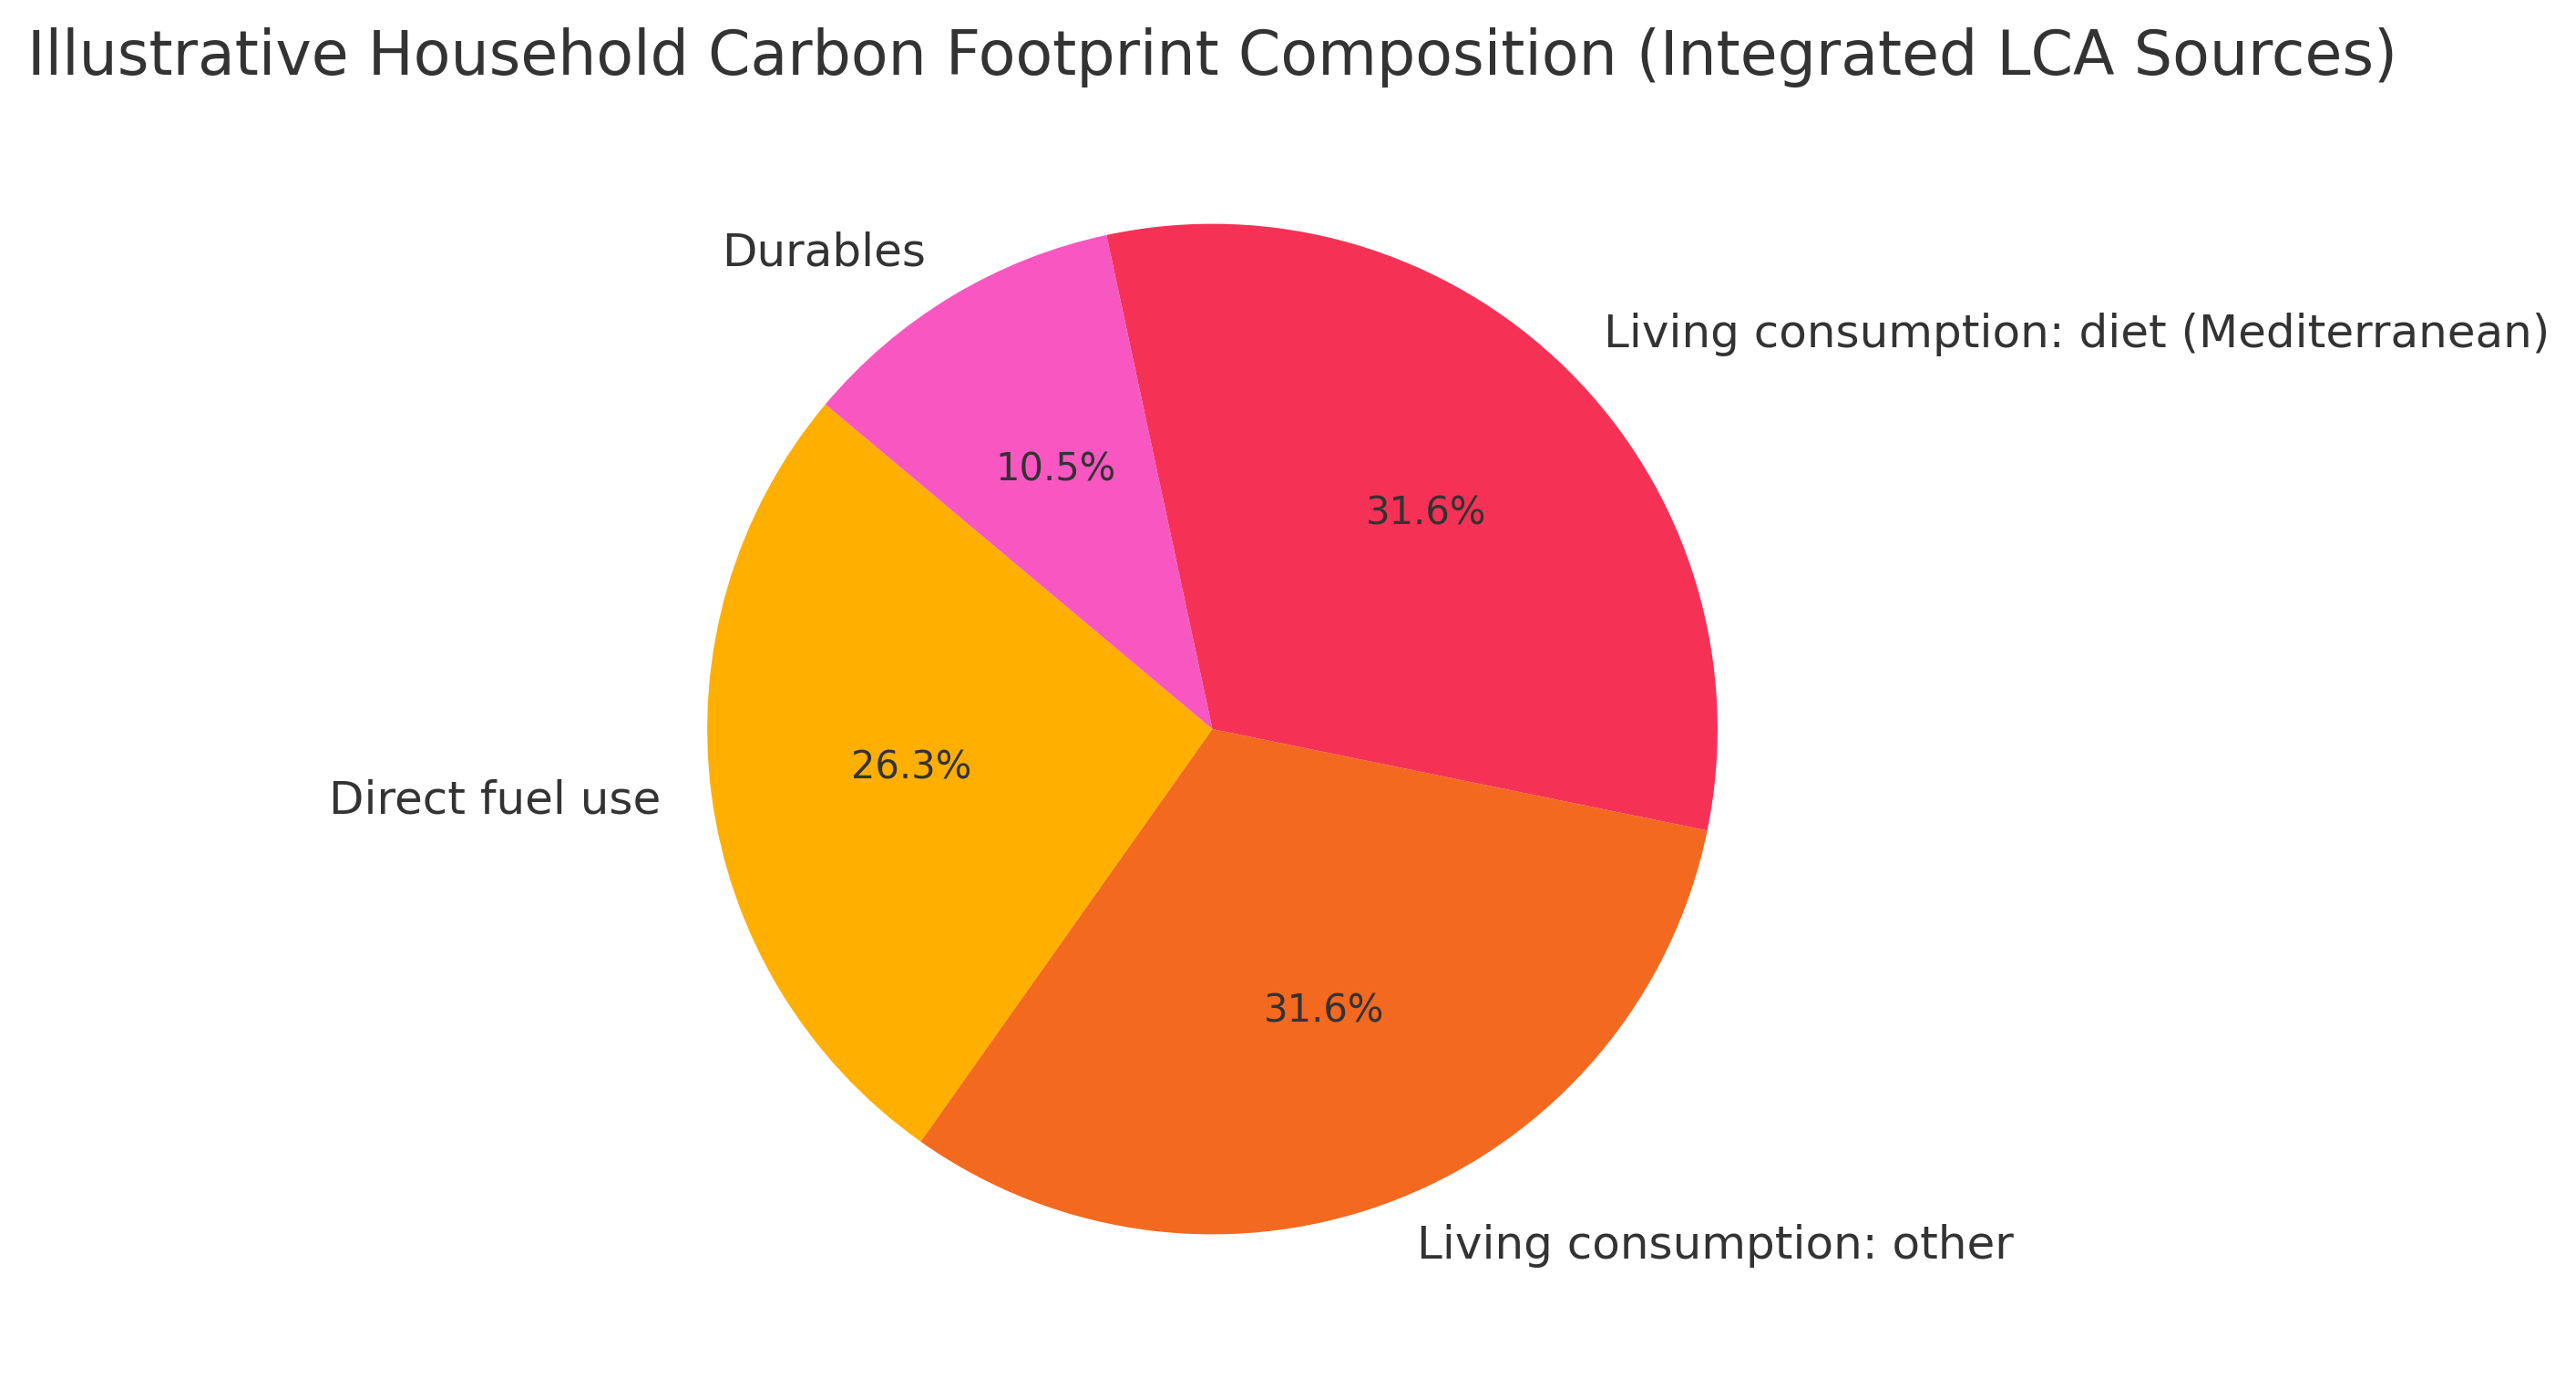
\includegraphics[width=0.8\linewidth]{LCA_pie_chart.png}
\caption{Relative contributions of household activities to carbon footprints}
\end{figure}

\subsection{Illustration of LCA with Comparative Insights from EEIOA}

Life cycle assessment (LCA) and environmentally extended input--output analysis (EEIOA) are two established methods for quantifying the carbon footprint of household consumption. While both approaches aim to capture direct and indirect greenhouse gas (GHG) emissions, they differ significantly in scope, resolution, and attribution of emissions. This section illustrates the application of LCA to household carbon footprints, integrating insights from Steubing et al. (2022), who compare LCA-based carbon footprints with those derived from EEIOA databases.

In the LCA approach, household carbon footprints are computed by summing emissions across all relevant activities and life cycle stages. The total household carbon footprint can be expressed as:
\begin{equation}
\text{CF}_{\text{total}} = \sum_d (F_{id} \cdot EF_d) 
+ \sum_f (C_{if} \cdot EF_f) 
+ \sum_j \left( \frac{C_{ij} \cdot EF_j}{L_j} \right)
+ \sum_a (M_{ia} \cdot EF_a)
- \sum_t (S_{it} \cdot CS_t)
\end{equation}
where $F_{id}$ is the fuel consumption for fuel type $d$, $C_{if}$ is the consumption of short-lived goods $f$, $C_{ij}$ is the consumption of durable goods $j$ with lifespan $L_j$, $M_{ia}$ is the material input for agricultural activity $a$, and $S_{it}$ is the sequestration from afforestation activity $t$. $EF$ and $CS$ denote emission factors and carbon stock, respectively.

Steubing et al. (2022) highlight that LCA-based carbon footprints typically provide a detailed, process-specific view, often including the life cycle impacts of capital goods and infrastructure. In contrast, EEIOA provides a macroeconomic perspective, covering the entire supply chain through national accounting frameworks. A key finding is that, despite theoretical expectations that EEIOA would yield higher carbon footprints due to the avoidance of truncation errors, LCA-based estimates can be higher in certain sectors. This discrepancy arises because LCA more comprehensively accounts for capital goods and specific life cycle stages, whereas EEIOA often omits the impacts of capital formation, as represented mathematically by the exclusion of gross fixed capital formation from the supply chain matrix:
\begin{equation}
\text{CF}_{\text{EEIOA}} = R (I - A)^{-1} y
\end{equation}
where $R$ is the vector of emission intensities, $A$ is the technology matrix, $I$ is the identity matrix, and $y$ is the final demand vector. In standard EEIOA practice, $y$ excludes capital goods destined for production.

Comparative analysis reveals that LCA is particularly effective in capturing emissions from long-lived assets and infrastructure-intensive activities, such as renewable energy installations, whereas EEIOA better reflects the systemic supply chain emissions associated with everyday consumption. This has critical implications for household carbon footprint assessments: neglecting either method's strengths risks underrepresenting key components of emissions. For instance, Steubing et al. (2022) report that for electricity, fossil-fuel-based power shows good alignment between LCA and EEIOA results, while renewable energy systems exhibit larger discrepancies due to the treatment of construction impacts in LCA.

Illustrating household carbon footprints using LCA not only clarifies the sources of emissions by activity and material flow but also exposes the limitations of relying on purely economic or monetary input--output models. The integrated perspective is essential for designing mitigation strategies that address both immediate consumption patterns and the long-term impacts of infrastructure and capital goods.

\subsection{Input-Output Matrix Model}

\subsubsection*{Measurement of Carbon Footprint Using I-O Matrix}

Household carbon footprints (HCF) are categorized into three tiers: \textit{Tier 1} (direct fuel combustion), \textit{Tier 2} (indirect emissions from purchased electricity and heating), and \textit{Tier 3} (indirect emissions from goods and services). An Input-Output (I-O) framework is employed to estimate these emissions systematically. This methodology follows the approach outlined in Matthews et al. (2008) and Long et al. (2019).

\subsubsection*{Input-Output Framework}
The total economic output required to satisfy final demand \( \mathbf{F} \) in an economy is derived from the fundamental balance equation of input-output analysis:
\begin{equation}
    \mathbf{X} = (\mathbf{I} - \mathbf{A})^{-1} \mathbf{F}
\end{equation}
where \( \mathbf{X} \) represents the total output vector across all sectors, \( \mathbf{A} \) is the technology coefficient matrix that defines the interdependencies between industries, and \( \mathbf{I} \) is the identity matrix. The term \( (\mathbf{I} - \mathbf{A})^{-1} \) is known as the Leontief inverse, which accounts for both direct and indirect production effects required to meet final demand.

\subsubsection*{Tier 1: Direct Emissions}
Tier 1 emissions result from the direct combustion of fuels by households, including natural gas, gasoline, and heating oil. These emissions are quantified using the emission coefficient matrix \( \mathbf{R} \), which is a diagonal matrix where each element \( r_{ii} \) denotes the emission intensity per unit of fuel consumption. Household fuel consumption is represented as a vector \( \mathbf{y} \), yielding direct emissions:
\begin{equation}
    \mathbf{E}_1 = \mathbf{R} \mathbf{y}
\end{equation}
where \( \mathbf{E}_1 \) captures emissions directly attributable to household fuel usage.

\subsubsection*{Tier 2: Indirect Energy Emissions}
Indirect emissions arise from electricity and heating consumption, which are not directly combusted within households but contribute to emissions at the production stage. The calculation follows:
\begin{equation}
    \mathbf{E}_2 = \mathbf{R} (\mathbf{I} + \mathbf{A}') \mathbf{y}
\end{equation}
where \( \mathbf{A}' \) is a subset of the input-output matrix specific to energy-producing industries. The emission intensity vector \( \mathbf{R} \) in this case reflects the carbon footprint of electricity and heat generation.

\subsubsection*{Tier 3: Indirect Supply Chain Emissions}
Traditional I-O models have been criticized, including by Matthews et al. (2008), for underestimating supply chain emissions due to the exclusion of imports and economic interactions beyond the primary production stage. To improve accuracy, we adopt an import-adjusted balance equation:
\begin{equation}
    \mathbf{X} = [(\mathbf{I} - \mathbf{M}) (\mathbf{I} - \mathbf{A})]^{-1} [(\mathbf{I} - \mathbf{M}) \mathbf{F} + \mathbf{EX}]
\end{equation}
where \( \mathbf{M} \) is the import-adjustment matrix that removes non-domestic contributions, ensuring that emissions are calculated based solely on domestic production. The term \( \mathbf{EX} \) represents exports, ensuring that emissions are assigned to domestic consumption rather than international trade.

Applying the emission intensity matrix \( \mathbf{D} \), the total indirect supply chain emissions are given by:
\begin{equation}
    \mathbf{E}_3 = \mathbf{D} [(\mathbf{I} - \mathbf{M}) (\mathbf{I} - \mathbf{A})]^{-1} [(\mathbf{I} - \mathbf{M}) \mathbf{F} + \mathbf{EX}]
\end{equation}
This formulation captures emissions embedded in the entire production and distribution chain, offering a more comprehensive estimation of the household carbon footprint.

\subsubsection*{Total Household Carbon Footprint}
The overall household carbon footprint integrates direct, indirect energy, and supply chain emissions:
\begin{equation}
    \mathbf{E}_{\text{total}} = \mathbf{E}_1 + \mathbf{E}_2 + \mathbf{E}_3
\end{equation}
This formulation aligns with recent advances in environmentally extended input-output models, refining emission estimations by incorporating full economic feedback loops and import corrections. The inclusion of trade-adjusted emissions ensures a more realistic and policy-relevant estimation of household contributions to carbon emissions, as emphasized by Long et al. (2019).
\subsection{Input-Output Matrix Model}

\subsubsection*{Measurement of Carbon Footprint Using I-O Matrix}

Household carbon footprints (HCF) are categorized into three tiers: \textit{Tier 1} (direct fuel combustion), \textit{Tier 2} (indirect emissions from purchased electricity and heating), and \textit{Tier 3} (indirect emissions from goods and services). An Input-Output (I-O) framework is employed to estimate these emissions systematically. This methodology follows the approach outlined in Matthews et al. (2008) and Long et al. (2019).

\subsubsection*{Input-Output Framework}
The total economic output required to satisfy final demand \( \mathbf{F} \) in an economy is derived from the fundamental balance equation of input-output analysis:
\begin{equation}
    \mathbf{X} = (\mathbf{I} - \mathbf{A})^{-1} \mathbf{F}
\end{equation}
where \( \mathbf{X} \) represents the total output vector across all sectors, \( \mathbf{A} \) is the technology coefficient matrix that defines the interdependencies between industries, and \( \mathbf{I} \) is the identity matrix. The term \( (\mathbf{I} - \mathbf{A})^{-1} \) is known as the Leontief inverse, which accounts for both direct and indirect production effects required to meet final demand.

\subsubsection*{Tier 1: Direct Emissions}
Tier 1 emissions result from the direct combustion of fuels by households, including natural gas, gasoline, and heating oil. These emissions are quantified using the emission coefficient matrix \( \mathbf{R} \), which is a diagonal matrix where each element \( r_{ii} \) denotes the emission intensity per unit of fuel consumption. Household fuel consumption is represented as a vector \( \mathbf{y} \), yielding direct emissions:
\begin{equation}
    \mathbf{E}_1 = \mathbf{R} \mathbf{y}
\end{equation}
where \( \mathbf{E}_1 \) captures emissions directly attributable to household fuel usage.

\subsubsection*{Tier 2: Indirect Energy Emissions}
Indirect emissions arise from electricity and heating consumption, which are not directly combusted within households but contribute to emissions at the production stage. The calculation follows:
\begin{equation}
    \mathbf{E}_2 = \mathbf{R} (\mathbf{I} + \mathbf{A}') \mathbf{y}
\end{equation}
where \( \mathbf{A}' \) is a subset of the input-output matrix specific to energy-producing industries. The emission intensity vector \( \mathbf{R} \) in this case reflects the carbon footprint of electricity and heat generation.

\subsubsection*{Tier 3: Indirect Supply Chain Emissions}
Traditional I-O models have been criticized, including by Matthews et al. (2008), for underestimating supply chain emissions due to the exclusion of imports and economic interactions beyond the primary production stage. To improve accuracy, we adopt an import-adjusted balance equation:
\begin{equation}
    \mathbf{X} = [(\mathbf{I} - \mathbf{M}) (\mathbf{I} - \mathbf{A})]^{-1} [(\mathbf{I} - \mathbf{M}) \mathbf{F} + \mathbf{EX}]
\end{equation}
where \( \mathbf{M} \) is the import-adjustment matrix that removes non-domestic contributions, ensuring that emissions are calculated based solely on domestic production. The term \( \mathbf{EX} \) represents exports, ensuring that emissions are assigned to domestic consumption rather than international trade.

Applying the emission intensity matrix \( \mathbf{D} \), the total indirect supply chain emissions are given by:
\begin{equation}
    \mathbf{E}_3 = \mathbf{D} [(\mathbf{I} - \mathbf{M}) (\mathbf{I} - \mathbf{A})]^{-1} [(\mathbf{I} - \mathbf{M}) \mathbf{F} + \mathbf{EX}]
\end{equation}
This formulation captures emissions embedded in the entire production and distribution chain, offering a more comprehensive estimation of the household carbon footprint.

\subsubsection*{Total Household Carbon Footprint}
The overall household carbon footprint integrates direct, indirect energy, and supply chain emissions:
\begin{equation}
    \mathbf{E}_{\text{total}} = \mathbf{E}_1 + \mathbf{E}_2 + \mathbf{E}_3
\end{equation}
This formulation aligns with recent advances in environmentally extended input-output models, refining emission estimations by incorporating full economic feedback loops and import corrections. The inclusion of trade-adjusted emissions ensures a more realistic and policy-relevant estimation of household contributions to carbon emissions, as emphasized by Long et al. (2019).

\subsection{Input-Output Matrix Model}

\subsubsection*{Measurement of Carbon Footprint Using I-O Matrix}

Household carbon footprints (HCF) are categorized into three tiers: \textit{Tier 1} (direct fuel combustion), \textit{Tier 2} (indirect emissions from purchased electricity and heating), and \textit{Tier 3} (indirect emissions from goods and services). An Input-Output (I-O) framework is employed to estimate these emissions systematically. This methodology follows the approach outlined in Matthews et al. (2008) and Long et al. (2019).

\subsubsection*{Input-Output Framework}
The total economic output required to satisfy final demand \( \mathbf{F} \) in an economy is derived from the fundamental balance equation of input-output analysis:
\begin{equation}
    \mathbf{X} = (\mathbf{I} - \mathbf{A})^{-1} \mathbf{F}
\end{equation}
where \( \mathbf{X} \) represents the total output vector across all sectors, \( \mathbf{A} \) is the technology coefficient matrix that defines the interdependencies between industries, and \( \mathbf{I} \) is the identity matrix. The term \( (\mathbf{I} - \mathbf{A})^{-1} \) is known as the Leontief inverse, which accounts for both direct and indirect production effects required to meet final demand.

\subsubsection*{Tier 1: Direct Emissions}
Tier 1 emissions result from the direct combustion of fuels by households, including natural gas, gasoline, and heating oil. These emissions are quantified using the emission coefficient matrix \( \mathbf{R} \), which is a diagonal matrix where each element \( r_{ii} \) denotes the emission intensity per unit of fuel consumption. Household fuel consumption is represented as a vector \( \mathbf{y} \), yielding direct emissions:
\begin{equation}
    \mathbf{E}_1 = \mathbf{R} \mathbf{y}
\end{equation}
where \( \mathbf{E}_1 \) captures emissions directly attributable to household fuel usage.

\subsubsection*{Tier 2: Indirect Energy Emissions}
Indirect emissions arise from electricity and heating consumption, which are not directly combusted within households but contribute to emissions at the production stage. The calculation follows:
\begin{equation}
    \mathbf{E}_2 = \mathbf{R} (\mathbf{I} + \mathbf{A}') \mathbf{y}
\end{equation}
where \( \mathbf{A}' \) is a subset of the input-output matrix specific to energy-producing industries. The emission intensity vector \( \mathbf{R} \) in this case reflects the carbon footprint of electricity and heat generation.

\subsubsection*{Tier 3: Indirect Supply Chain Emissions}
Traditional I-O models have been criticized, including by Matthews et al. (2008), for underestimating supply chain emissions due to the exclusion of imports and economic interactions beyond the primary production stage. To improve accuracy, we adopt an import-adjusted balance equation:
\begin{equation}
    \mathbf{X} = [(\mathbf{I} - \mathbf{M}) (\mathbf{I} - \mathbf{A})]^{-1} [(\mathbf{I} - \mathbf{M}) \mathbf{F} + \mathbf{EX}]
\end{equation}
where \( \mathbf{M} \) is the import-adjustment matrix that removes non-domestic contributions, ensuring that emissions are calculated based solely on domestic production. The term \( \mathbf{EX} \) represents exports, ensuring that emissions are assigned to domestic consumption rather than international trade.

Applying the emission intensity matrix \( \mathbf{D} \), the total indirect supply chain emissions are given by:
\begin{equation}
    \mathbf{E}_3 = \mathbf{D} [(\mathbf{I} - \mathbf{M}) (\mathbf{I} - \mathbf{A})]^{-1} [(\mathbf{I} - \mathbf{M}) \mathbf{F} + \mathbf{EX}]
\end{equation}
This formulation captures emissions embedded in the entire production and distribution chain, offering a more comprehensive estimation of the household carbon footprint.

\subsubsection*{Total Household Carbon Footprint}
The overall household carbon footprint integrates direct, indirect energy, and supply chain emissions:
\begin{equation}
    \mathbf{E}_{\text{total}} = \mathbf{E}_1 + \mathbf{E}_2 + \mathbf{E}_3
\end{equation}
This formulation aligns with recent advances in environmentally extended input-output models, refining emission estimations by incorporating full economic feedback loops and import corrections. The inclusion of trade-adjusted emissions ensures a more realistic and policy-relevant estimation of household contributions to carbon emissions, as emphasized by Long et al. (2019).
\section{Illustrative Application of the Input-Output Model}

Following the formal derivation of the environmentally extended input-output (EEIO) model, this section presents an illustrative application of the framework to household carbon footprint estimation. The aim is to operationalize the Leontief-based formulation:
\[
\mathbf{E} = \mathbf{C} (\mathbf{I}-\mathbf{A})^{-1} \mathbf{F}
\]
where $\mathbf{F}$ denotes the final demand vector, here represented by annual household consumption expenditure by category; ${(\mathbf{I}-\mathbf{A})}^{-1}$ is the Leontief inverse, capturing direct and indirect production requirements to satisfy $\mathbf{F}$; $\mathbf{C}$ is the vector of direct emission intensities (kg CO$_{2}$e per unit output).

In this illustration, pre-calculated environmentally extended emission intensities (kg CO$_{2}$e per euro spent) are applied to household consumption data for France, Spain, and Germany for 2021. These intensities represent the aggregated effect of $\mathbf{C} {(\mathbf{I}-\mathbf{A})}^{-1}$ and are derived from the EXIOBASE multi-regional input-output (MRIO) model, as accessed via Climatiq.io. The method aligns with the tier-3 comprehensive accounting approach discussed in Matthews et al.~(2008), Long et al.~(2019), and Sheng et al.~(2024).

\subsection{Data and Methodology}

Household final consumption expenditure data were obtained from Eurostat and supplementary sources, converted to euros at the 2021 average exchange rate (1 USD = 0.85 EUR). Table~\ref{tab:efactors} summarizes the emission intensities applied.

\begin{table}[h]
\centering
\caption{Spend-Based Emission Factors (EXIOBASE via Climatiq.io)}
\label{tab:efactors}
\begin{tabular}{@{}ll@{}}
\toprule
\textbf{Category} & \textbf{Emission Factor (kgCO$_{2}$e/€)}\\
\midrule
Housing, water, electricity, gas & 0.30\\
Food and non-alcoholic beverages & 0.48\\
Transport & 0.40\\
Other goods and services & 0.18\\
Recreation and culture & 0.20\\
Restaurants and hotels & 0.45\\
Furnishings and household equipment & 0.25\\
Health & 0.20\\
Alcoholic beverages and tobacco & 0.42\\
Clothing and footwear & 0.25\\
Communications & 0.15\\
Education & 0.15\\
\bottomrule
\end{tabular}
\end{table}

For each country $c$, and for each category $i$, the household carbon footprint is calculated as:
\[
E_{i,c} = F_{i,c} \cdot EF_i
\]
where:
\begin{itemize}
    \item $F_{i,c}$ is the household expenditure in euros for category $i$ in country $c$;
    \item $EF_i$ is the spend-based emission factor for category $i$;
    \item $E_{i,c}$ is the resulting emissions (kg CO$_{2}$e).
\end{itemize}

\subsection{Explicit Calculation Example}

For France, the household expenditure on food and non-alcoholic beverages is:
\[
F_{\text{food,FR}} = 1.322 \times 10^9 \cdot 0.139 = 183.8 \times 10^9 \text{ EUR}
\]
The corresponding emissions are:
\[
E_{\text{food,FR}} = 183.8 \times 10^9 \cdot 0.48 = 88.2 \times 10^6 \ \text{tonnes CO}_{2}\text{e}
\]

Analogously, calculations are performed for all categories and countries.

\subsection{Results}

\begin{table}[h]
\centering
\caption{Estimated Household Carbon Footprints by Category (Million Tonnes CO$_{2}$e)}
\label{tab:results}
\begin{tabular}{@{}lccc@{}}
\toprule
\textbf{Category} & \textbf{France} & \textbf{Spain} & \textbf{Germany}\\
\midrule
Housing, water, electricity, gas & 109.5 & 50.4 & 137.3\\
Food and non-alcoholic beverages & 88.2 & 47.1 & 100.7\\
Transport & 66.6 & 30.4 & 94.1\\
Other goods and services & 29.8 & 12.8 & 42.3\\
Recreation and culture & 20.4 & 9.1 & 34.1\\
Restaurants and hotels & 37.3 & 37.3 & 32.3\\
Furnishings and household equipment & 16.2 & 8.5 & 31.4\\
Health & 11.1 & 6.1 & 20.1\\
Alcoholic beverages and tobacco & 22.8 & 12.8 & 27.1\\
Clothing and footwear & 10.9 & 6.0 & 17.1\\
Communications & 5.0 & 2.8 & 6.2\\
Education & 1.0 & 1.5 & 2.2\\
\midrule
\textbf{Total} & \textbf{419.0} & \textbf{223.0} & \textbf{544.9}\\
\bottomrule
\end{tabular}
\end{table}

\subsection{Discussion}

This illustration demonstrates how the IO model framework, when combined with spend-based emission intensities, yields a comprehensive household carbon footprint that captures both direct and indirect emissions. The method is widely applied due to its ability to integrate complex supply chain interactions, incorporate international trade adjustments (Long et al.~2019), and support policy-relevant analyses of consumption-based emissions (Matthews et al.~2008; Sheng et al.~2024).

\begin{table}[h]
\centering
\caption{Household Expenditure Share by Category (\% of Total, 2021)}
\label{tab:appendix_expenditure}
\begin{tabular}{lccc}
\hline
\textbf{Category} & \textbf{France} & \textbf{Spain} & \textbf{Germany}\\
\hline
Housing, water, electricity, gas & 27.6 & 24.3 & 25.5\\
Food and non-alcoholic beverages & 13.9 & 14.2 & 11.7\\
Transport & 12.6 & 11.0 & 13.1\\
Other goods and services & 12.5 & 10.3 & 13.1\\
Recreation and culture & 7.7 & 6.6 & 9.5\\
Restaurants and hotels & 6.2 & 12.0 & 4.0\\
Furnishings, household equipment & 4.9 & 4.9 & 7.0\\
Health & 4.2 & 4.4 & 5.6\\
Alcoholic beverages, tobacco & 4.1 & 4.4 & 3.6\\
Clothing and footwear & 3.3 & 3.5 & 3.8\\
Communications & 2.5 & 2.7 & 2.3\\
Education & 0.5 & 1.4 & 0.8\\
\hline
\end{tabular}
\end{table}

\section{Bibliometric Analysis of Household Carbon Footprint Studies Using Input-Output Models}

\subsection{Methodology}

This bibliometric analysis follows the methodological approach used by Sheng et al. (2024). Publications were retrieved from Scopus, using search terms related to household carbon footprint, input-output, EEIO, and environmentally extended, comprising 208 unique publications on household carbon footprint estimation using input-output (IO) models, including environmentally extended input-output (EEIO) and multi-regional input-output (MRIO) frameworks. The dataset covers publications from 2008 to 2025. Duplicate records were removed using DOI and EID identifiers. Python (pandas and matplotlib) was used for data cleaning and visualization. Metrics examined include temporal publication trends, lead author contributions, co-authorship patterns, and source journals with their publishing countries.

\subsection{Results}

\subsubsection{Temporal Publication Trends}

The annual distribution of publications (Figure~\ref{fig:Publications}) shows steady growth in the field since 2010, with notable peaks in 2020 (27 publications), 2021 (26 publications), and sustained activity through 2024 (23 publications). This trend is consistent with findings reported by Sheng et al. (2024).

\begin{figure}[h]
\centering
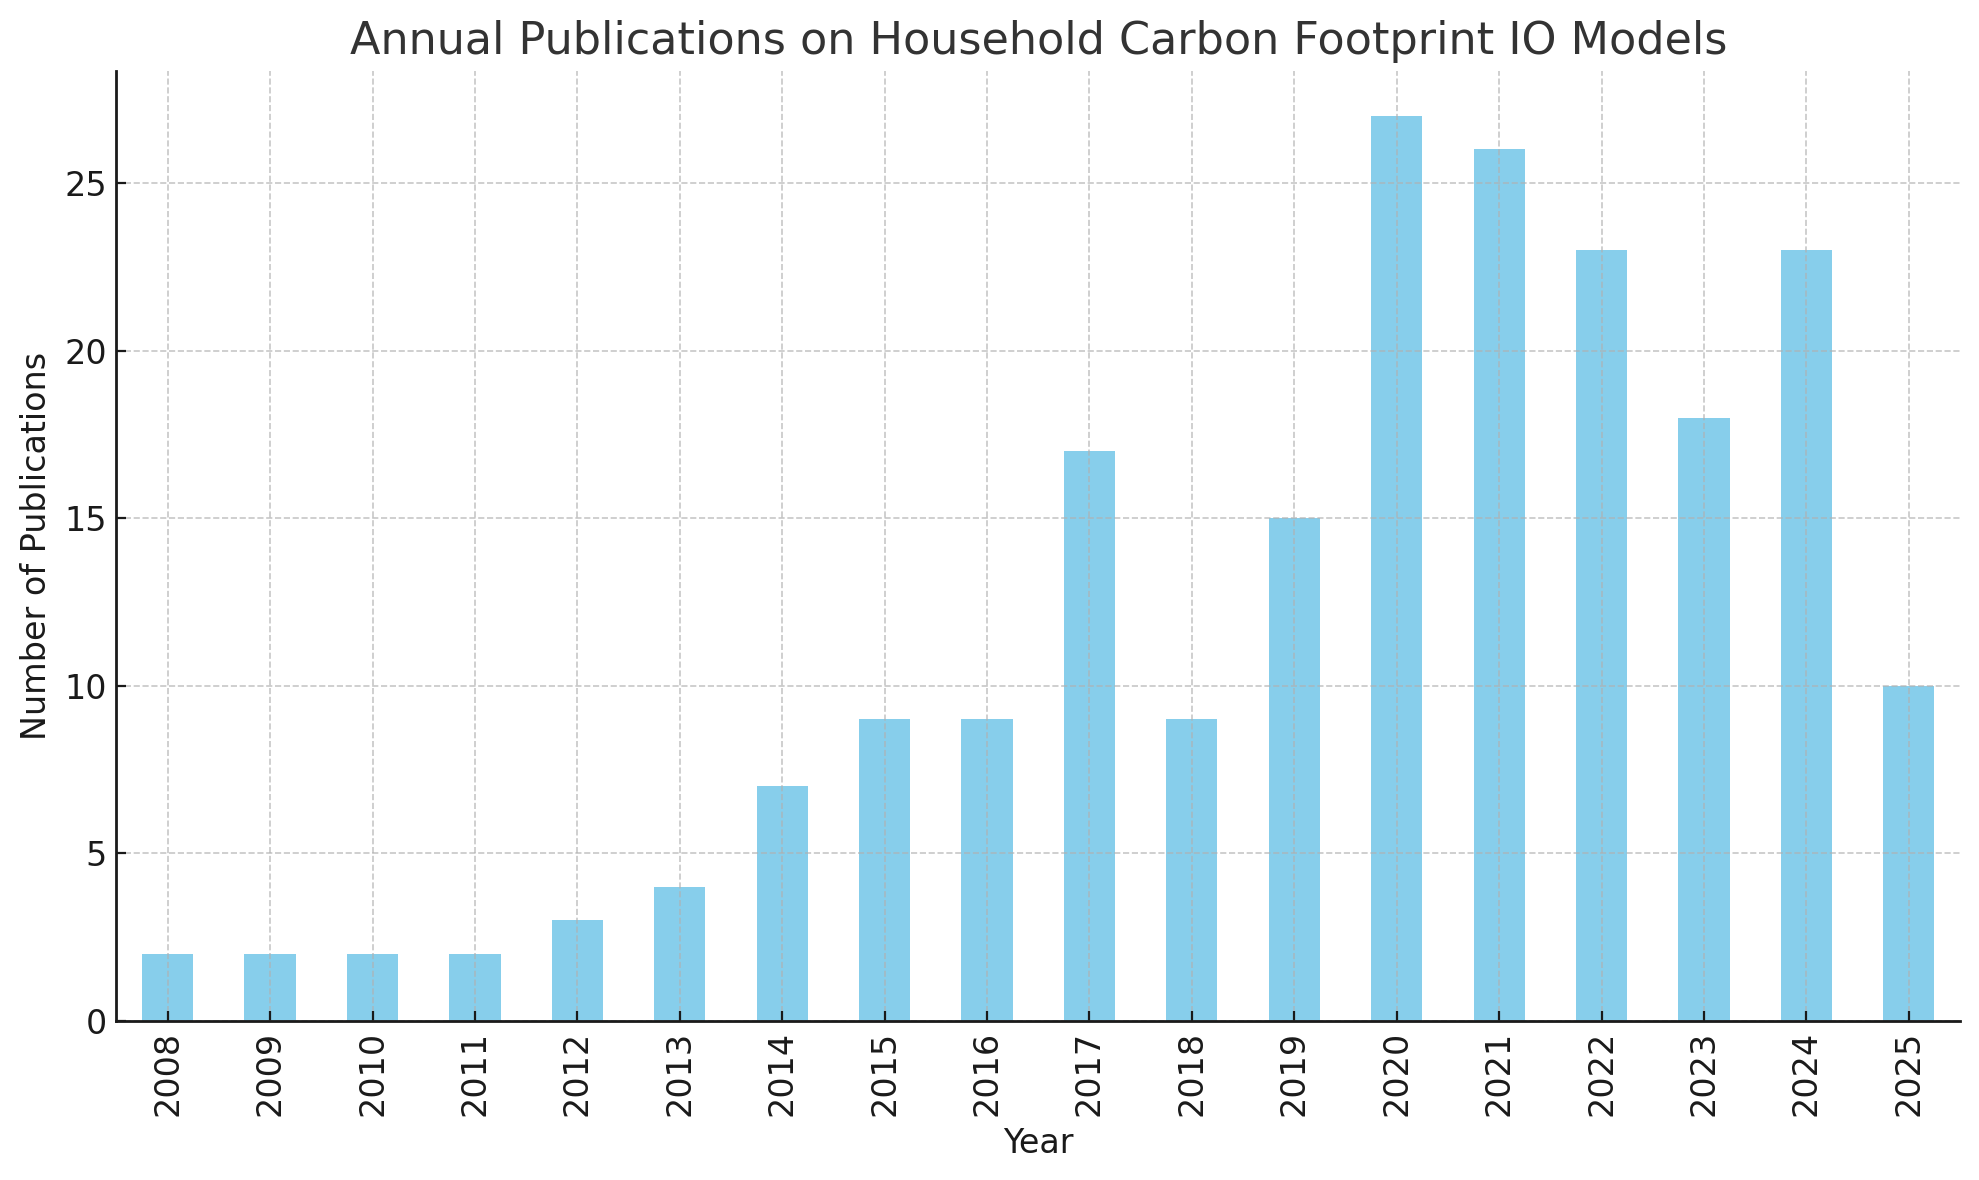
\includegraphics[width=0.7\textwidth]{Publications.png}
\caption{Annual publications on household carbon footprint using input-output models (2008--2025)}
\label{fig:Publications}
\end{figure}

\subsubsection{Lead Author Contributions}

The analysis of lead authorship indicates that a small number of researchers have contributed repeatedly as lead authors in this field (Table~\ref{tab:lead_authors}). 

\begin{table}[h]
\centering
\caption{Top lead authors, number of publications, and affiliations.}
\label{tab:lead_authors_affiliations}
\begin{tabular}{@{}lrl@{}}
\hline
\textbf{Lead Author} & \textbf{Publications} & \textbf{Affiliation} \\
\hline
Long Y. & 9 & Beijing Institute of Technology, China \\
Shigetomi Y. & 5 & Kyushu University, Japan \\
Ivanova D. & 4 & Norwegian University of Science and Technology, Norway \\
Ala-Mantila S. & 4 & Aalto University, Finland \\
Druckman A. & 3 & University of Surrey, UK \\
Liu X. & 3 & Chinese Academy of Sciences, China \\
Owen A. & 2 & University of Leeds, UK \\
Zhong H. & 2 & Chinese Academy of Sciences, China \\
Chen G. & 2 & Norwegian University of Science and Technology, Norway \\
Christis M. & 2 & University of Antwerp, Belgium \\
\hline
\end{tabular}
\end{table}


\begin{figure}[h]
\centering
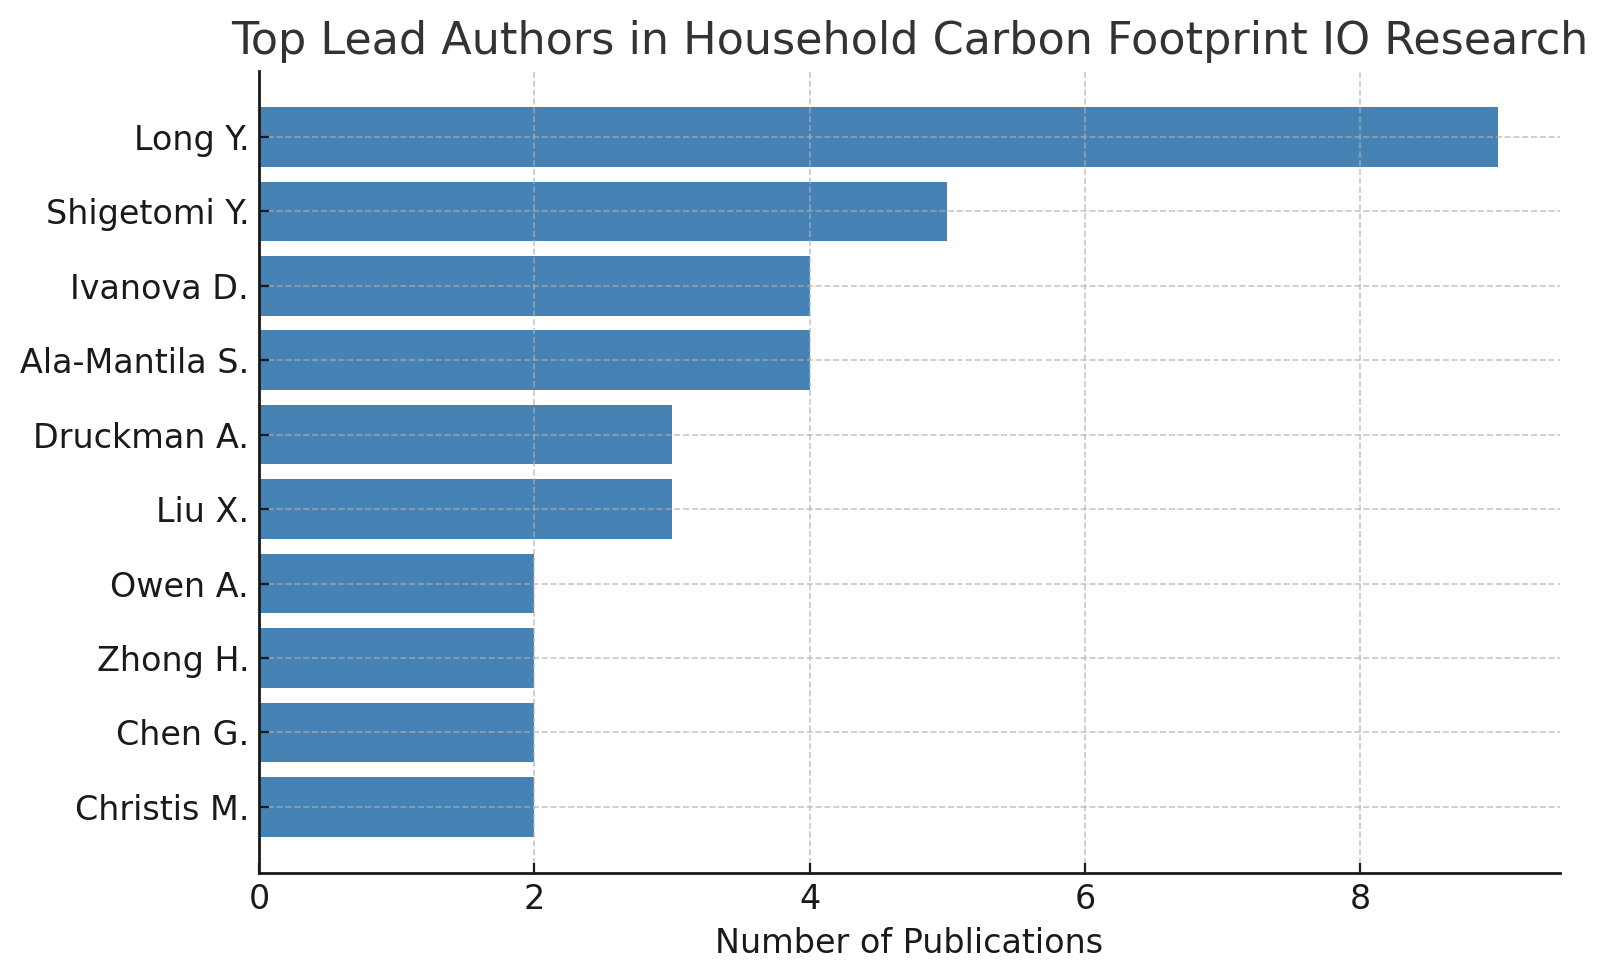
\includegraphics[width=0.7\textwidth]{Authors.png}
\caption{Top lead authors in household carbon footprint IO research}
\label{fig:lead_authors}
\end{figure}

\subsubsection{Co-authorship Patterns}

The distribution of co-authorship (Figure~\ref{fig:coauthorship}) demonstrates the collaborative nature of the field, with most publications involving multiple authors.

\begin{figure}[h]
\centering
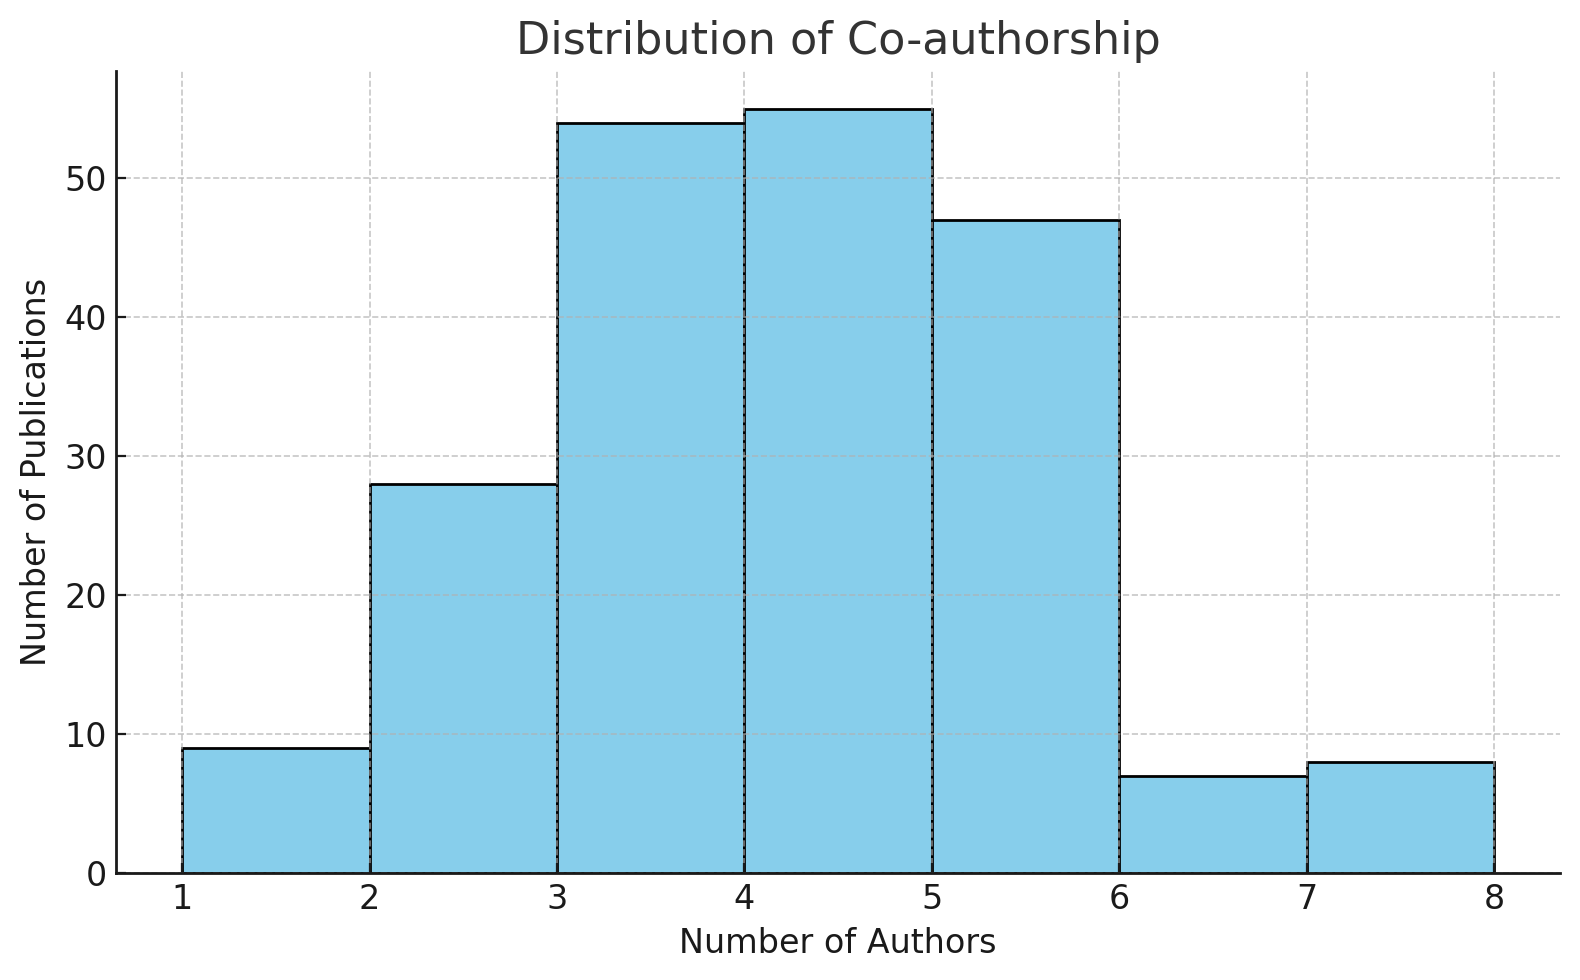
\includegraphics[width=0.7\textwidth]{Coauthors.png}
\caption{Distribution of co-authorship in household carbon footprint IO publications}
\label{fig:coauthorship}
\end{figure}

\subsubsection{Top Source Journals}

Table~\ref{tab:journal_countries} presents the top journals in terms of publication count, along with their publishing countries. The results highlight a strong presence of journals published in the Netherlands (Elsevier) and the USA.

\begin{table}[h]
\centering
\caption{Top Source Journals, Number of Publications, and Publishing Countries}
\label{tab:journal_countries}
\begin{tabular}{lll}
\hline
\textbf{Journal} & \textbf{Publications} & \textbf{Country} \\
\hline
Journal of Cleaner Production & 24 & UK / Netherlands \\
Ecological Economics & 16 & Netherlands \\
Environmental Research Letters & 14 & UK \\
Journal of Industrial Ecology & 11 & USA \\
Resources, Conservation and Recycling & 11 & Netherlands \\
Science of the Total Environment & 11 & Netherlands \\
Energy Policy & 9 & Netherlands \\
Sustainability (Switzerland) & 8 & Switzerland \\
Journal of Environmental Management & 8 & Netherlands \\
Environmental Science and Technology & 5 & USA \\
\hline
\end{tabular}
\end{table}

\subsection{Discussion}

The analysis reveals the significant growth of input-output based household carbon footprint studies, particularly after 2010. A small group of researchers, such as Long Y. and Shigetomi Y., have been especially productive. The field shows a strong collaborative character, as evidenced by the prevalence of multi-authored publications. The majority of research outputs are concentrated in leading journals published in the Netherlands, the USA, and the UK, reflecting the central role of these countries in disseminating knowledge on this topic.

\section*{The Hakenes \& Schliephake Model}

Traditional methods for estimating household carbon footprints attribute emissions based on direct consumption or financial ownership in emitting industries. However, they often ignore the market feedback loops triggered by individual decisions — such as how a household reducing demand might simply shift that demand to other consumers or investors.

The model developed by Hakenes and Schliephake (2024) addresses this issue through a general equilibrium framework. By embedding both product and financial markets, the model assigns carbon footprints based not only on what households consume or invest in, but also on the spillover effects of those choices across the economy. This consequentialist approach attempts to capture the true marginal impact of household behavior on aggregate emissions.

\section{Deriving the Household Footprint in a One-Industry Economy}

We consider a simplified version of the model developed by Hakenes and Schliephake (2024), focusing on an economy with a single industry. A representative good is produced using capital as the only input. Firms operate under constant returns to scale, with a marginal cost of production $c$. Let $Q$ denote the aggregate quantity produced and consumed, and $I$ the total capital invested. Given the linear technology, we have:

\[
I = cQ.
\]

Each unit of the good generates emissions $x$, which aggregates both production-related and consumption-related emissions. Thus, total emissions in the economy are given by:

\[
X = xQ.
\]

\subsection*{Firms and Capital Market}

Firms raise capital $I$ from households and produce output $Q$. After selling the output at price $P$, they repay investors using the liquidation value $\lambda$ and a noise term $\varepsilon$, which follows a normal distribution with zero mean and variance $\sigma^2$. The return on investment is:

\[
r = \frac{P}{c} + \lambda + \varepsilon.
\]

Profits are distributed to investors in proportion to their capital contributions. Firms operate competitively, so expected profits are zero in equilibrium.

\subsection*{Household Optimization Problem}

Household $h$ is endowed with wealth $w$ and allocates it between investment $i_h$ and consumption $q_h$. The portion not invested yields a risk-free return $r_f$. The budget constraint is:

\[
m_h = r i_h + r_f(w - i_h) - P q_h,
\]

where $m_h$ is the leftover wealth after investment and consumption. The household derives utility from consumption and terminal wealth. The expected utility function is given by:

\[
U_h = \mathbb{E} \left[ -e^{-\alpha \left( a q_h - \frac{b}{2}q_h^2 + m_h - xQ \right)} \right],
\]

where $a$ represents the marginal utility of the first unit of the good, $b > 0$ captures diminishing marginal utility, $\alpha$ is the coefficient of absolute risk aversion, and $xQ$ reflects the disutility from global emissions.

Substituting $m_h$ into the utility function and linearizing expectations due to the exponential-normal structure, we obtain:

\[
\mathbb{E}[U_h] = -\exp \left\{ -\alpha \left[ (a - P)q_h - \frac{b}{2}q_h^2 + r_f w + \left( \frac{P}{c} + \lambda - r_f \right)i_h - \frac{\alpha}{2} \sigma^2 i_h^2 - xQ \right] \right\}.
\]

\subsection*{Market Equilibrium and Footprint Derivation}

To calculate the household's consequentialist footprint, we compare the equilibrium outcome with and without household $h$. In equilibrium, the market clears:

\[
Q = q_h + (n - 1) q_{-h}, \quad I = i_h + (n - 1) i_{-h}, \quad I = cQ.
\]

Other households maximize the same utility, taking $P$ as given. Their optimal demand and investment are derived from the first-order conditions:

\[
q_{-h} = \frac{a - x - P}{b}, \quad i_{-h} = \frac{1}{\alpha \sigma^2} \left( \frac{P}{c} + \lambda - r_f \right).
\]

Substituting these into the equilibrium conditions and solving, we obtain the aggregate quantity:

\[
Q = \phi q_h + (1 - \phi) \frac{i_h}{c} + \text{(terms independent of } h),
\]

where the weighting parameter $\phi$ is defined as:

\[
\phi = \frac{b}{b + c^2 \alpha \sigma^2}.
\]

This weight determines how the household’s choices affect equilibrium quantities and, consequently, emissions. The consequentialist footprint of household $h$ is defined as the marginal impact of their participation on total emissions:

\[
fp_h = x \left( Q(q_h, i_h) - Q(0, 0) \right) = x \left( \phi q_h + (1 - \phi) \frac{i_h}{c} \right).
\]


The parameter $\phi$ captures the relative influence of consumption and investment. When the financial asset is risk-free ($\sigma^2 = 0$), we obtain $\phi = 1$, and the entire footprint is attributed to consumption. Conversely, if consumption utility is linear ($b = 0$), then $\phi = 0$, and the footprint depends entirely on investment. This formulation ensures full accounting of emissions across households:

\[
\sum_h fp_h = xQ = X.
\]
\section{Derivation of the Weighting Parameter \( \boldsymbol{\phi} \)}

To derive the footprint weighting parameter \( \boldsymbol{\phi} \), we begin with the assumption that aggregate output \( Q \) is produced by a linear technology using capital \( I \) with constant marginal cost \( c \). Hence,
\[
Q = \frac{I}{c}.
\]

The total capital in the market is supplied by \( n \) households. We distinguish a representative household \( h \) from the remaining \( n - 1 \) households, and denote their investment and consumption decisions by \( (i_h, q_h) \) and \( (i_{-h}, q_{-h}) \), respectively.

In equilibrium, market clearing implies:
\[
Q = q_h + (n - 1) q_{-h}, \quad I = i_h + (n - 1) i_{-h}, \quad I = cQ.
\]

Substituting into the identity \( I = cQ \), we obtain:
\[
i_h + (n - 1) i_{-h} = c \left( q_h + (n - 1) q_{-h} \right).
\]

Now consider how the quantity \( Q \) changes when household \( h \) changes its behavior. Holding the other households' behavior fixed, the marginal effect of \( h \)'s consumption and investment on output is given by the total differential:
\[
\frac{\partial Q}{\partial q_h} = 1, \quad \frac{\partial Q}{\partial i_h} = \frac{1}{c}.
\]

However, these effects are attenuated by the endogenous reactions of other households. If household \( h \) increases consumption \( q_h \), market price \( P \) rises. Other households respond by lowering their own consumption \( q_{-h} \) and adjusting their investment \( i_{-h} \) to the new return. Conversely, if \( h \) increases investment \( i_h \), the capital supply rises, which reduces price and affects others' choices.

We now derive the explicit behavioral responses.

The other households' optimal consumption satisfies:
\[
\frac{\partial \mathbb{E}[U_{-h}]}{\partial q_{-h}} = 0 \quad \Rightarrow \quad a - x - b q_{-h} - P = 0,
\]
which yields:
\[
q_{-h} = \frac{a - x - P}{b}.
\]

Their optimal investment satisfies:
\[
\frac{\partial \mathbb{E}[U_{-h}]}{\partial i_{-h}} = 0 \quad \Rightarrow \quad \frac{P}{c} + \lambda - r_f - \alpha \sigma^2 i_{-h} = 0,
\]
so that:
\[
i_{-h} = \frac{1}{\alpha \sigma^2} \left( \frac{P}{c} + \lambda - r_f \right).
\]

Now insert these behavioral responses into the aggregate equilibrium conditions:
\[
Q = q_h + (n - 1) \left( \frac{a - x - P}{b} \right), \quad I = i_h + (n - 1) \left( \frac{1}{\alpha \sigma^2} \left( \frac{P}{c} + \lambda - r_f \right) \right).
\]

Combining these with \( Q = \frac{I}{c} \), we solve for the dependence of \( Q \) on \( q_h \) and \( i_h \). Define the partial footprint of household \( h \) as the difference in total output caused by its activity:
\[
fp_h = x \left( Q(q_h, i_h) - Q(0, 0) \right).
\]

Linearizing \( Q \) in \( q_h \) and \( i_h \), and denoting the resulting coefficients as footprint weights, we obtain:
\[
fp_h = x \left( \phi q_h + (1 - \phi) \frac{i_h}{c} \right),
\]
where
\[
\phi = \frac{b}{b + c^2 \alpha \sigma^2}.
\]

This expression reflects how much of the household’s carbon footprint is attributed to consumption versus investment. It arises from the equilibrium interactions between price responses and household behavioral elasticities in both the product and capital markets.

\section{Comparative Statics of the Weighting Parameter \( \boldsymbol{\phi} \)}

We now investigate how the footprint weighting parameter \( \boldsymbol{\phi} \), defined as
\[
\boldsymbol{\phi} = \frac{b}{b + c^2 \alpha \sigma^2},
\]
responds to changes in the underlying structural parameters of the model.

Differentiating \( \boldsymbol{\phi} \) with respect to the coefficient of absolute risk aversion \( \alpha \), we obtain
\[
\frac{\partial \boldsymbol{\phi}}{\partial \alpha} = -\frac{b c^2 \sigma^2}{(b + c^2 \alpha \sigma^2)^2} < 0.
\]
This implies that as households become more risk-averse, the footprint share attributed to consumption declines, while the relative importance of investment decisions increases.

With respect to the volatility of financial returns, captured by \( \sigma^2 \), we find
\[
\frac{\partial \boldsymbol{\phi}}{\partial \sigma^2} = -\frac{b c^2 \alpha}{(b + c^2 \alpha \sigma^2)^2} < 0.
\]
An increase in financial risk similarly reduces \( \boldsymbol{\phi} \), shifting the footprint burden from consumption to investment channels.

Finally, consider the effect of changing the curvature of the utility function through the parameter \( b \). Differentiation yields
\[
\frac{\partial \boldsymbol{\phi}}{\partial b} = \frac{c^2 \alpha \sigma^2}{(b + c^2 \alpha \sigma^2)^2} > 0.
\]
A higher value of \( b \), indicating stronger diminishing marginal utility from consumption, increases the share of the footprint attributed to consumption activities.

In sum, the weighting parameter \( \boldsymbol{\phi} \) is decreasing in both risk aversion and return volatility, and increasing in the concavity of consumption preferences. These results highlight how the relative responsibility of consumption and investment for carbon emissions is endogenous to household behavior and financial risk, making the model responsive to empirical variation across households or economies.

\section{Empirical Illustration: Application of the Single-Industry Model}

Here, the simplified version of the Hakenes and Schliephake (2024) model is applied to the U.S. wheat market, using USDA data from 2010 to 2016. Production volumes serve as a proxy for quantity supplied, while total domestic use approximates quantity demanded. Farm prices are taken as observed average annual prices.

To estimate supply behavior, an ordinary least squares (OLS) regression of price is fitted on observed production, yielding the empirical supply curve. In the empirical illustration, the demand curve is specified as linear and downward sloping. Its slope is calibrated using average values from the dataset, consistent with observed market behavior in the U.S. wheat sector. While the curve is not estimated directly via regression (due to data limitations on price responsiveness), it reflects a stylized elasticity based on domain knowledge. This contrasts with the supply curve, which is estimated using OLS on observed price and production data. We simulate the 2016–2017 wheat supply shock, during which production declined by 15.6\%. The intersection of the two curves provide the empirical equilibrium quantities and prices before and after the 2016–2017 supply shock. This is modeled by proportionally shifting the supply curve upward. Equilibrium price and quantity before and after the shock are obtained by solving the intersection between the demand curve and the respective supply curves.


\subsection*{Carbon Footprint Estimation under Empirical Supply Curve}

We compute the carbon footprint associated with each equilibrium using an emission factor of 10.88 kg CO\textsubscript{2}e per bushel (based on FAO and USDA estimates).

\begin{table}[ht]
\centering
\begin{tabular}{lccc}
\toprule
\textbf{Scenario} & \textbf{Quantity} & \textbf{Price} & \textbf{Carbon Footprint} \\
\textbf{USDA data} & \textbf{(million bushels)} & \textbf{(USD)} & \textbf{(million kg CO\textsubscript{2}e)} \\
\midrule
Before Shock  & 2100.71 & 5.58 & 22859.68 \\
After Shock & 2068.38 & 5.82 & 22500.32 \\
\midrule
\textbf{Change} & \textemdash& \textemdash& \textbf{-359.36} \\
\bottomrule
\end{tabular}
\caption{Carbon footprint before and after the supply shock using real market data.}
\end{table}

\subsection*{Carbon Footprint Estimation under Theoretical Supply Curve}

To simulate the same supply shock within the Hakenes and Schliephake (2024) framework, the demand curve from the empirical estimation was retained. However, instead of using a supply curve estimated via ordinary least squares, a theoretically derived supply curve was constructed based on model assumptions. In this approach, firms were assumed to raise capital from households, who in turn optimally allocate their investments under risk.

The equilibrium supply curve in this setup is derived from the market-clearing condition and the household's optimal investment response under uncertainty, and takes the form:
\[
P(Q) = c(r_f - \lambda) + \frac{c^2 \alpha \sigma^2}{n - 1} Q,
\]
where \( c \) denotes the marginal cost of production, \( r_f \) the risk-free rate, \( \lambda \) the liquidation value of capital, \( \alpha \) the coefficient of absolute risk aversion, \( \sigma^2 \) the variance of investment returns, and \( n \) the total number of households. 

This expression yields a linear and upward-sloping supply curve. The theoretical supply curve applied in this illustration was constructed using parameter values selected to reflect realistic conditions in the U.S. wheat and financial markets during the study period. The marginal cost of production was assumed to be $c = 4$, which is consistent with per-bushel production costs observed in U.S. wheat farming and allows the resulting equilibrium prices to align with historical market levels. The risk-free rate was set to $r_f = 0.05$, corresponding to the average yield on 10-year U.S. Treasury bonds between 2010 and 2016. The liquidation value of capital was taken as $\lambda = 0.01$, reflecting the reduced resale value of farm-specific capital such as machinery or equipment. The coefficient of absolute risk aversion was assumed to be $\alpha = 0.5$, a value that captures moderate household risk sensitivity consistent with empirical estimates from investment literature. The volatility of investment returns was specified as $\sigma = 0.4$, implying a variance of $\sigma^2 = 0.16$, which falls within the range typically observed for U.S. agricultural investments and related financial instruments. Finally, the number of households was assumed to be $n = 100{,}000$, representing an approximation of the number of wheat-producing farms in the United States during the relevant years. These parameter values were used to generate a supply curve that reflects theoretical investment behavior under risk, providing a basis for comparison with the empirically estimated curve, and the intercept reflects the opportunity cost of capital. The new equilibrium values were obtained by solving the intersection of this supply curve with the demand curve used previously.

By solving the intersection of this supply curve with the same demand curve used in the empirical case, equilibrium values for price and quantity were obtained both before and after the simulated shock. The corresponding carbon footprints were then computed using the same emissions factor of 10.88 kg CO\textsubscript{2}e per bushel.

\begin{table}[ht]
\centering
\begin{tabular}{lccc}
\toprule
\textbf{Scenario} & \textbf{Quantity} & \textbf{Price} & \textbf{Carbon Footprint} \\
\textbf{Theory} & \textbf{(million bushels)} & \textbf{(USD)} & \textbf{(million kg CO\textsubscript{2}e)} \\
\midrule
Before Shock & 2112.36 & 5.69 & 22983.46 \\
After Shock   & 2095.13 & 5.85 & 22808.35 \\
\midrule
\textbf{Change} & \textemdash& \textemdash & \textbf{-175.11} \\
\bottomrule
\end{tabular}
\caption{Model-based carbon footprint before and after the supply shock.}
\end{table}

\subsection*{Structural Sources of Difference in Emissions Outcomes}

Although the same demand curve was used in both the empirical and theoretical approaches, the estimated reduction in carbon footprint differed considerably. The empirical estimation yielded a reduction of 359.36 million kg CO\textsubscript{2}e, while the theoretical model predicted a more modest reduction of 175.11 million kg CO\textsubscript{2}e.

This difference can be attributed entirely to the way supply was modeled. In the empirical estimation, the supply curve was estimated via OLS using observed data on price and quantity. This approach captured market behavior as it appeared in the historical record but did not account for underlying decision-making under uncertainty or equilibrium responses. In contrast, the theoretical supply curve was derived from the model’s structural assumptions, incorporating risk preferences, investment volatility, and optimal capital allocation. It reflected how households would respond to market changes under forward-looking behavior, leading to a more muted response in output and, correspondingly, in emissions.

Additionally, the theoretical model introduced a consequentialist perspective by assigning carbon responsibility based on the marginal impact of a household's consumption or investment. In doing so, it internalized substitution effects and capital reallocation, which were not accounted for in the empirical estimation. As a result, while the same emissions formula was applied in both cases, the theoretical model predicted a smaller footprint change due to the buffering effects of equilibrium adjustments. This difference underscores the importance of integrating behavioral dynamics into footprint assessment, particularly when evaluating the impact of shocks or policy interventions.

\section{Results}

\section{Discussion}

\section{Conclusion}

\newpage
\begin{thebibliography}{9}
% Bibliography entries
\end{thebibliography}

% Statement of authorship
\newpage
\thispagestyle{empty}
\section*{Statement of authorship}
I hereby confirm that the work presented has been performed and interpreted solely by myself except for where I explicitly identified the contrary.

\vspace{2cm}
Date: \underline{\hspace{5cm}}

\vspace{1cm}
Signature: \underline{\hspace{5cm}}
\end{document}
